%%
%% This is file `sample-manuscript.tex',
%% generated with the docstrip utility.
%%
%% The original source files were:
%%
%% samples.dtx  (with options: `manuscript')
%% 
%% IMPORTANT NOTICE:
%% 
%% For the copyright see the source file.
%% 
%% Any modified versions of this file must be renamed
%% with new filenames distinct from sample-manuscript.tex.
%% 
%% For distribution of the original source see the terms
%% for copying and modification in the file samples.dtx.
%% 
%% This generated file may be distributed as long as the
%% original source files, as listed above, are part of the
%% same distribution. (The sources need not necessarily be
%% in the same archive or directory.)
%%
%% Commands for TeXCount
%TC:macro \cite [option:text,text]
%TC:macro \citep [option:text,text]
%TC:macro \citet [option:text,text]
%TC:envir table 0 1
%TC:envir table* 0 1
%TC:envir tabular [ignore] word
%TC:envir displaymath 0 word
%TC:envir math 0 word
%TC:envir comment 0 0
%%
%%
%% The first command in your LaTeX source must be the \documentclass command.
%%%% Small single column format, used for CIE, CSUR, DTRAP, JACM, JDIQ, JEA, JERIC, JETC, PACMCGIT, TAAS, TACCESS, TACO, TALG, TALLIP (formerly TALIP), TCPS, TDSCI, TEAC, TECS, TELO, THRI, TIIS, TIOT, TISSEC, TIST, TKDD, TMIS, TOCE, TOCHI, TOCL, TOCS, TOCT, TODAES, TODS, TOIS, TOIT, TOMACS, TOMM (formerly TOMCCAP), TOMPECS, TOMS, TOPC, TOPLAS, TOPS, TOS, TOSEM, TOSN, TQC, TRETS, TSAS, TSC, TSLP, TWEB.
% \documentclass[acmsmall]{acmart}

%%%% Large single column format, used for IMWUT, JOCCH, PACMPL, POMACS, TAP, PACMHCI
% \documentclass[acmlarge,screen]{acmart}

%%%% Large double column format, used for TOG
% \documentclass[acmtog, authorversion]{acmart}

%%%% Generic manuscript mode, required for submission
%%%% and peer review
\documentclass[sigconf]{acmart}
%% Fonts used in the template cannot be substituted; margin 
%% adjustments are not allowed.
%%
%% \BibTeX command to typeset BibTeX logo in the docs
\AtBeginDocument{%
  \providecommand\BibTeX{{%
    \normalfont B\kern-0.5em{\scshape i\kern-0.25em b}\kern-0.8em\TeX}}}

\usepackage{amsmath, amssymb, amsfonts}% mathematical symbols and the like
\usepackage{amsthm}% definitions, theorems, etc.
\usepackage[colorinlistoftodos]{todonotes}% marking open todos in text/on margins
\usepackage{subfig}% multi-part figures with separate captions per part
\usepackage{url}% render URLs correctly and make them clickable through the hyperref package
\usepackage{longtable}% tables that span multiple pages
\usepackage{booktabs}% tables that actually look good
\usepackage[nolist]{acronym}% consistently use acronyms
\usepackage{algpseudocode} % Algorithms
\usepackage{pdfpages}
\usepackage{tikz}
\usetikzlibrary{trees,fit,arrows.meta,shapes,calc,decorations.pathmorphing}
\usepackage{rotating}
\usepackage{float}
\usepackage{pgfgantt} %Ganttchart
\newacro{SCITE}[SCITE]{``Single Cell Inference of Tumor Evolution''}
\newacro{SNP}[SNP]{Single-Nucleotide Polymorphism}
\newacro{infSCITE}[$\infty$SCITE]{Infinity-SCITE}
\newacro{MCMC}[MCMC]{Monte Carlo Markov Chain}
\newacro{FPGA}[FPGA]{Field-Programmable Gate Array}
\newacro{HPC}[HPC]{High-Performance Computing}
\newacro{RNG}[RNG]{random number generator}
\newacro{CPU}[CPU]{Central Processing Unit}
\newacro{GPU}[GPU]{Graphics Processing Unit}
\newacro{TOST}[TOST]{``Two One-Sided t-Tests''}
\newacro{ffSCITE}[ffSCITE]{``fabulously fast SCITE''}
\newacro{ffSCITE}[bbSCITE]{``bit-based SCITE''}
%\newacro{BRAM}[BRAM]{block RAM}
\newacro{BRAM}[RAM blocks]{on-chip RAM blocks}
\newacro{URNG}[URNG]{uniform random number generator}
\newacro{II}[II]{initiation interval}
\newacro{FF}[FF]{flip-flop}
\newacro{LUT}[LUT]{look-up table}
\newacro{MLAB}[MLAB]{memory logic array block}
\newacro{BSP}[BSP]{board support package}
\newacro{DSP}[DSP]{digital signal processor}
\newacro{HLS}[HLS]{high-level synthesis}


%%%%%%%%%%%%%%%
% Custom floats
%%%%%%%%%%%%%%%

%\newfloat{algorithm}{thp}{lop}
%l\floatname{algorithm}{Algorithm}

%% Rights management information.  This information is sent to you
%% when you complete the rights form.  These commands have SAMPLE
%% values in them; it is your responsibility as an author to replace
%% the commands and values with those provided to you when you
%% complete the rights form.

\copyrightyear{2023}
\acmYear{2023}
\setcopyright{cc}
\setcctype{by-sa}
\acmConference[HEART 2023]{The International Symposium on Highly Efficient Accelerators and Reconfigurable Technologies 2023}{June 14--16, 2023}{Kusatsu, Japan}
\acmBooktitle{The International Symposium on Highly Efficient Accelerators and Reconfigurable Technologies 2023 (HEART 2023), June 14--16, 2023, Kusatsu, Japan}
\acmDOI{10.1145/3597031.3597050}
\acmISBN{979-8-4007-0043-9/23/06}

%%
%% For managing citations, it is recommended to use bibliography
%% files in BibTeX format.
%%
%% You can then either use BibTeX with the ACM-Reference-Format style,
%% or BibLaTeX with the acmnumeric or acmauthoryear sytles, that include
%% support for advanced citation of software artefact from the
%% biblatex-software package, also separately available on CTAN.
%%
%% Look at the sample-*-biblatex.tex files for templates showcasing
%% the biblatex styles.
%%

%%
%% The majority of ACM publications use numbered citations and
%% references.  The command \citestyle{authoryear} switches to the
%% "author year" style.
%%
%% If you are preparing content for an event
%% sponsored by ACM SIGGRAPH, you must use the "author year" style of
%% citations and references.
%% Uncommenting
%% the next command will enable that style.
%%\citestyle{authoryear}

%%
%% end of the preamble, start of the body of the document source.
\begin{document}

%%
%% The "title" command has an optional parameter,
%% allowing the author to define a "short title" to be used in page headers.
\title[]{Mutation Tree Reconstruction of Tumor Cells on FPGAs Using a Bit-Level Matrix Representation}

%%
%% The "author" command and its associated commands are used to define
%% the authors and their affiliations.
%% Of note is the shared affiliation of the first two authors, and the
%% "authornote" and "authornotemark" commands
%% used to denote shared contribution to the research.
\author{Jan-Oliver Opdenhövel}
\affiliation{
  \institution{Paderborn University, Paderborn Center for Parallel Computing}
  \city{Paderborn}
  \country{Germany}
}
\email{joo@mail.uni-paderborn.de}
\orcid{0000-0003-2314-2784}

\author{Christian Plessl}
\affiliation{
  \institution{Paderborn University, Paderborn Center for Parallel Computing}
  \city{Paderborn}
  \country{Germany}
}
\email{plessl@uni-paderborn.de}
\orcid{0000-0001-5728-9982}

\author{Tobias Kenter}
\affiliation{
  \institution{Paderborn University, Paderborn Center for Parallel Computing}
  \city{Paderborn}
  \country{Germany}
}
\email{kenter@uni-paderborn.de}
\orcid{0000-0002-5088-0267}

%%
%% By default, the full list of authors will be used in the page
%% headers. Often, this list is too long, and will overlap
%% other information printed in the page headers. This command allows
%% the author to define a more concise list
%% of authors' names for this purpose.
\renewcommand{\shortauthors}{Opdenhövel, Plessl, Kenter}

%%
%% The abstract is a short summary of the work to be presented in the
%% article.
\begin{abstract}
    Reconstructing the mutation history of a cancer cell in the form of a phylogenetic tree 
    from noisy genome sequencing data requires a likelihood model and a search or optimization strategy. The \ac{SCITE} software performs such a search via Monte Carlo Markov Chains that explore and evaluate different random update operations on a current candidate tree.
    In this work, we present an FPGA accelerator design (denoted as \ac{ffSCITE}) that implements all required operations with deterministic latency as bit-operations on a matrix representation. The largest design updates and counts 36100 set bits in each clock cycle and thus outperforms the original single-threaded software reference by up to 80$\times$.
\end{abstract}

%%
%% The code below is generated by the tool at http://dl.acm.org/ccs.cfm.
%% Please copy and paste the code instead of the example below.
%%
\begin{CCSXML}
<ccs2012>
   <concept>
       <concept_id>10010520.10010521.10010542.10010543</concept_id>
       <concept_desc>Computer systems organization~Reconfigurable computing</concept_desc>
       <concept_significance>500</concept_significance>
       </concept>
    <concept>
       <concept_id>10010405.10010444.10010450</concept_id>
       <concept_desc>Applied computing~Bioinformatics</concept_desc>
       <concept_significance>500</concept_significance>
       </concept>
   <concept>
       <concept_id>10010583.10010682.10010684</concept_id>
       <concept_desc>Hardware~High-level and register-transfer level synthesis</concept_desc>
       <concept_significance>100</concept_significance>
       </concept>
 </ccs2012>
\end{CCSXML}

\ccsdesc[500]{Computer systems organization~Reconfigurable computing}
\ccsdesc[500]{Applied computing~Bioinformatics}
\ccsdesc[100]{Hardware~High-level and register-transfer level synthesis}

%%
%% Keywords. The author(s) should pick words that accurately describe
%% the work being presented. Separate the keywords with commas.
\keywords{FPGA, Monte Carlo Markov Chain (MCMC), Bit-level parallelism, SYCL, oneAPI}

%%
%% This command processes the author and affiliation and title
%% information and builds the first part of the formatted document.
\maketitle
\acresetall

%\todo[inline]{What about open directions and related work? I have no open directions that appear interesting to me, and I have done little research on other stuff. Should I write something about that? And if so, how much? -> Yes, no paper completely without these two aspects. 
%Open directions can also serve as inspiration for other people, so the actual intention to do it yourself is not a necessity.
%Maybe there is no such closely related work that it needs its own section, but we can have a general discussion as part of the introduction. }

\section{Introduction}
% Context / Motivation
\acp{FPGA} have been used with great success for the acceleration of workloads from bioinformatics. A particular focus has been on sequence alignment~\cite{yu-kw-03a,zh-ta-07a,ja-la-08a}, where datatypes with few bits for nucleotides or amino acids allowed to create highly parallel customized datapaths. 
% in particular short read alignment~\cite{yu-kw-03a,zh-ta-07a}
Rapid advancements in genome sequencing technology and basic analysis techniques as the identification of genome differences in the \ac{SNP} are a foundation for ever more sophisticated analysis procedures on top of them. One such direction is reconstructing the mutation history of cancer cells based on single-cell sequencing. 

% Challenge
The software approach published as \ac{SCITE}~\cite{tree2016} is by itself again a computationally demanding workload that can profit from FPGA acceleration. However, the involved algorithms and data structures are different from the foundational components of sequence alignment. The \ac{SCITE} software reference~\cite{tree2016} maintains and modifies a tree structure representing a hypothesis for the mutation history that is regularly transformed into a matrix structure to calculate the likelihood of the current hypothesis. As the involved tree traversals and modifications generally involve a dynamic number of sequential sub-steps, it is inherently challenging to create a well-utilized computation pipeline with parallelism for them.

In this work, we present the first \ac{FPGA} accelerator for \ac{SCITE} and resolve the challenge of tree data structures by reformulating the tree updates as parallel binary operations on equivalent bit-matrix representations. Our further contributions include:
\begin{itemize}
    \item A meta-pipeline that overlaps the evolution of several independent \acp{MCMC} to obtain full utilization of the datapath.
    \item Support for different problem sizes at runtime with design parameterization at compile time.
    \item End-to-end speedups of up to 80$\times$ against a sequential CPU reference and a performance model that explains the measured throughput.
    \item A comparison with an idealized CPU performance proxy for the throughput-critical likelihood calculation step.
\end{itemize}
\section{Application Background}
\label{sec:introduction}

\ac{SCITE} \cite{tree2016} is an algorithm and code from the domain of bioinformatics. It solves the real-world problem where multiple cells are extracted from a patient's tumor and a practitioner wants to analyze which mutations are present in the tumor and lead to its current state. There are single-cell sequencers available that can analyze the genome of a single cell and report whether certain genes are in their common, unmutated form or whether they are mutated. However, these results are often noisy. Sometimes, the sequencers report a mutation that is not present, sometimes they fail to find a mutation, and sometimes the gene is lost in the process and therefore no statement about its mutation status can be made. The sequencing output is represented as a matrix $D[cell][gene]$ with one row for every cell that is analyzed and one column for every gene that is considered. The matrix entries are either 0 for no mutation, 1 for a mutation, and 2 for missing data. As stated before, this reported mutation matrix $D$ contains errors due to the sequencing process and often does not represent a biologically plausible mutation history of the analyzed cells. We define $E$ as the true mutation matrix for these cells.
%We, therefore, assume that there is a also true mutation matrix $E$ which contains the actual state of the cells. %We do not know $E$ and it is the task of \ac{SCITE} to find it.
The \ac{SCITE} approach to reconstruct $E$ builds on the one hand on a likelihood model presented in the next paragraph that quantifies how well a candidate for $E$ fits to the observations encoded in $D$, and on the other hand on a mutation model that defines a search space of possible candidates for $E$, described afterwards.

\subsection{Likelihood Model}

%In order to find $E$, certain assumptions are made. First of all, w
For the likelihood model, we assume that the errors the sequencer makes for every entry of $D$ are independent of another. If the data for an entry is not missing, we assume that there is a probability for false positives called $\alpha \in [0,1]$ and a probability for false negatives called $\beta \in [0,1]$. Conversely, the probability for a true positive is $1-\beta$ and the probability for a true negative is $1-\alpha$. Formally, this means that we have the following for every cell $c$ and gene $g$:
\begin{align}
    \mathbb{P}(D[c][g] = 1 \mid E[c][g] = 0 \wedge D[c][g] \neq 2) &= \alpha \\
    \mathbb{P}(D[c][g] = 0 \mid E[c][g] = 0 \wedge D[c][g] \neq 2) &= 1-\alpha \\
    \mathbb{P}(D[c][g] = 0 \mid E[c][g] = 1 \wedge D[c][g] \neq 2) &= \beta \\
    \mathbb{P}(D[c][g] = 1 \mid E[c][g] = 1 \wedge D[c][g] \neq 2) &= 1-\beta
\end{align}
With this probability model, we can build a likelihood function that measures the likelihood of a given candidate for $E$ by multiplying the probabilities for every matrix entry:
\begin{align}
    \Lambda(E, D) := \prod_{c \in C} \prod_{g \in G} \begin{cases}
        1-\alpha & D[c][g] = 0 \wedge E[c][g] = 0 \\
        \beta & D[c][g] = 0 \wedge E[c][g] = 1 \\
        \alpha & D[c][g] = 1 \wedge E[c][g] = 0 \\
        1-\beta & D[c][g] = 1 \wedge E[c][g] = 1 \\
        1 & D[c][g] = 2
    \end{cases}
\end{align}
%We can therefore refine the task of \ac{SCITE} to find the most likely true mutation matrix $E$ for a given input mutation matrix $D$.
The task of \ac{SCITE} is to find the most likely true mutation matrix $E$ for a given input mutation matrix $D$.
%\todo[inline]{When readers look at the algorithm at this point, the descendant matrix (and underlying mutation tree) is not clear. We should probably move the next paragraph before this one, i.e. first there are candidate matrices E that obey to the underlying assumptions of a mutation tree, then we rate them how plausible they are w.r.t. D and the sequencer error rates.}

\subsection{Mutation Tree Model}

\begin{figure}[tbh]
    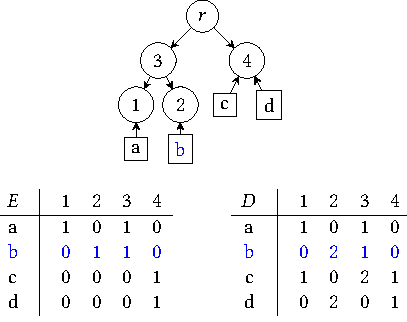
\includegraphics{figures/mutation_tree.pdf}

    \Description{A mutation tree with one root and four gene nodes, as well as four attached cells. Below, there are the corresponding true and noisy mutation matrices.}
    \caption{An example of a mutation tree, and related mutation matrices $E$ and $D$. The node $r$ represents the initial, unmutated state, the round nodes with numeric labels represent mutations of individual genes in the tree, and the square nodes with letter labels represent cells that are attached to the tree nodes. The true mutation matrix $E$ and the noisy mutation matrix $D$ have one row for each cell and one column for each gene. Exemplarily, the highlighted cell \textcolor{emph}{b} contains mutations in genes 2 and 3 (second row of $E$), but during readout, the information on gene 2 was lost (entry 2 in second row of $D$).}
    \label{fig:mutation_tree}
\end{figure}

%Even with this refined goal, there are still many possible versions of $E$. In order to restrict the possible true mutation matrices even further, 
In order to define a search space for plausible mutation matrices, the so-called "infinite sites assumption" is made in SCITE. It assumes that every gene mutates exactly once in the history of the tumor and that the first cell with such a mutation passes it down to all of its descendants that are created via cell division. This assumption allows to model the mutation history as a tree. Every node represents a mutation state and is labeled with a gene. The root $r$ represents the initial, unmutated state of the genome and every child adds a mutation of its label gene to its parent's state. In other words, a gene $g$ is mutated in the state of a node $v$ iff there is a node $w$ on the path from $r$ to $v$ with the label $g$. 
%Lastly, we attach our cells to nodes in the tree, which means that we assume the mutation state of the attachment node for this cell. 
During the cell-extraction process, samples from any node in the mutation tree can be encountered, which is modeled by attaching cells to tree nodes.
%The tree and the cell attachments together describe a candidate for $E$ which can be evaluated with the likelihood function. 
%Since we want to maximize the likelihood function, we always pick the most likely attachment node for every cell. 
Fig.~\ref{fig:mutation_tree} gives an example how of a mutation tree with respective $E$ and $D$ may look like. During the sequencing stage, errors are introduced from $E$ to $D$, and during the reconstruction phase, we look for an $E$ that has the highest likelihood w.r.t. to $D$ and at the same time can be modeled with a mutation history that forms a tree.
While $E$ is only completely defined by the combination of mutation tree and cell attachment, \ac{SCITE} actually explores the candidate space for mutation trees and calculates the likelihood of each tree by identifying the most likely attachment for each cell in each evaluation step.

\subsection{Search Procedure}

%\ac{SCITE}, as stated earlier, is a \ac{MCMC} algorithm:
The search procedure to explore candidate mutation trees is a \acf{MCMC}.
It starts with a randomly generated tree and iteratively applies random modifications to it. If the resulting tree, together with the most likely attachments, is more likely to be correct than the previous tree, it is accepted as the new solution. If the new tree is less likely to be correct, a random threshold between 0 and 1 is drawn. If the ratio of the proposed likelihood to the current likelihood is lower than this threshold, the modification is rejected. This kernel loop of modifying the tree, computing its likelihood, and deciding on the new solution is then repeated multiple times and also restarted with new trees. For statistical details on the convergence of this search procedure, we refer to \citeauthor{tree2016} \cite{tree2016}. %\todo{is this interesting at this point?} Note that in their implementation, the moves are performed via pointer operations on a tree data structure, which is then transformed into a so-called ancestor matrix in every step to calculate the likelihood.

%With every step, the current tree converges to the most likely solution. For the statistical details, see \citeauthor{tree2016} \cite{tree2016}.

\section{FPGA design approach}
\label{sec:approach}

In this section, we present the \ac{FPGA} design denoted as \ac{ffSCITE} in terms of overall kernel structure, data representation, updates of mutation tree candidates, and parallel likelihood calculation. Although written with a specific implementation in mind, these design aspects are largely independent of the target FPGA architecture and used tool chain.

\subsection{Kernel Structure}
\label{sec:kernel_structure}

\begin{figure}[tbh]
    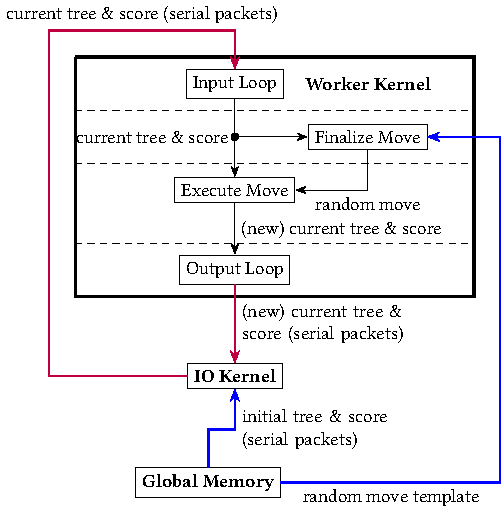
\includegraphics{figures/design.pdf}
    \Description{A block diagram with one nodes called ``Global Memory,'' ``IO Kernel,'' and ``Worker Kernel.'' The worker kernel is further subdivided into the blocks, ``Input Loop,'' ``Finalize Move,'' ``Execute Move,'' and ``Output Loop.''}
    \caption{Block diagram of the \acs{FPGA} design of \acs{ffSCITE}. The IO kernel and the worker kernel are connected via pipes, colored in violet, and the kernels access the global memory via load-store units, colored in blue. The sections separated by the dashed lines inside the worker kernel run in parallel and use/forward the values from the previous stage.}
    \label{fig:design}
\end{figure}

The general \ac{FPGA} design that realizes the \ac{MCMC} algorithm is illustrated in Fig.~\ref{fig:design} and contains a worker kernel and an IO kernel. These kernels are circularly connected using pipes realized as on-chip FIFO buffers. The IO kernel sends the current tree and its score to the worker kernel and with a design-specific latency, the worker kernel sends the result back to the IO kernel. Each transfer is done sequentially in several packets since a pipe with a sufficient bitwidth to transfer a full tree in one cycle would use excessive routing resources and would not be utilized in each cycle anyway. The worker kernel receives the current tree and its score with an input loop. Then, the kernel decides how to modify the tree. In order to save resources for a random number generator on the FPGA and since little off-chip bandwidth is used by the rest of the design, random move templates are pre-computed on the host. Before kernel invocation, they are transferred to the global memory of the accelerator card and streamed in and finalized with the knowledge of the current tree inside the worker kernel.
%We have previously computed the random numbers for this on the \ac{FPGA}, but the required pseudo-random number generator was a major bottleneck for the design. We have eliminated this bottleneck by precomputing random move templates on the host and storing them in the global memory of the accelerator card. The worker kernel only loads those templates from memory and finalizes them with the knowledge of the current tree. 
%\todo[inline]{Simplify by directly presenting the current version without the \emph{previously}.} 
Once the suggested move is decided, the ``Execute Move'' step executes the move, computes the likelihood score of the proposed tree, and decides whether the proposed tree is accepted as the new tree. As stated earlier, a proposed tree is accepted if it has a higher likelihood than the current tree or if the ratio of the proposed and the current likelihood is above a random threshold. This threshold is also fetched from global memory as part of the move template. The updated tree is fed back to the IO kernel. 
%It also internally stores the most likely tree encountered by the worker kernel and writes it back to global memory once the execution is finished.
%\tobias{Now, the updated tree could be directly fed back into input stage of the worker kernel. However, the latency for executing the move is higher than the inverse throughput of the worker kernel. Therefore, to avoid idle bubbles in the pipeline, moves on other, independent trees from other \acl{MCMC} are executed in an overlapping sequence meanwhile. To this end, the output loop sends the resulting tree back to the IO kernel, which schedules a configurable number of other, independent trees to the worker kernel before feeding the previous one back to the worker. The IO kernel also keeps track of the globally most likely candidate tree encountered by the worker kernel and writes it back to global memory once the execution is finished.}

These four parts, the input loop, the move finalization, the tree modification and scoring, and the output loop can work independently and form a meta-pipeline. The worker kernel can therefore process multiple chains at once, which is exploited by the IO kernel. It assumes a certain capacity for the worker kernel and initially feeds a corresponding number of chains into the worker kernel. Then, the previous outputs of the worker kernel are fed back into the loop, which maintains the occupation of the worker kernel despite relatively high latency of individual steps. Once the requested chain steps were executed, the output states are discarded and if more initial states are available, those are fed into the worker kernel instead of the previous output. Otherwise, the worker kernel is flushed and execution halts. The worker kernel also keeps track of the most likely candidate tree encountered so far and writes it back to global memory once the execution is finished.

\subsection{Ancestor and descendant matrices}
\label{subsec:ancestor_matrix}

\begin{figure}[tbh]
    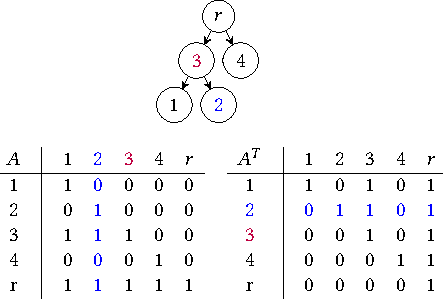
\includegraphics{figures/ancestor_matrix.pdf}

    \Description{The mutation tree from Fig.~\ref{fig:mutation_tree}, without the attached cell nodes, and the corresponding ancestor and descendant matrices below.}
    \caption{The mutation tree from Fig.~\ref{fig:mutation_tree} with the corresponding ancestor matrix $A$ and the descendant matrix $A^T$. The highlighted column \textcolor{emph}{2} in the ancestor matrix contains an entry $1$ for all nodes on the path from the root $r$ to the given node \textcolor{emph}{2}, i.e. $A[r][2] = A[3][2] = A[2][2] = 1$. Its transpose in $A^T$ is related to the mutation matrix $E$ in Fig.~\ref{fig:mutation_tree}: The first two rows are identical except for the inclusion of the root node since the cells $a$ and $b$ are attached to nodes 1 and 2, respectively. However, the fourth row of $A^T$ appears in the third and fourth row of $E$ since both $c$ and $d$ are attached to node 4, and the third row of $A^T$ does not appear in $E$ since no cell is attached to node 3.
    % Its transpose in $A^T$ is -- except for the inclusion of the root node -- identical to the mutation matrix $E$ in Fig.~\ref{fig:mutation_tree}. Note however the differences between the two matrices: column \textcolor{emph2}{3} in the ancestor matrix $A$ represents node \textcolor{emph2}{3} in the tree, which has no counterpart in the mutation matrix $E$ in Fig.~\ref{fig:mutation_tree}, because no cell is attached to it. In contrast, the mutation matrix $E$ in Fig.~\ref{fig:mutation_tree} contains two identical columns for two cells attached to node 4, whereas the ancestor matrix $A$ has one unique ancestry vector for node 4.}
    }
    \label{fig:ancestor_matrix}
\end{figure}

The main innovation in \ac{ffSCITE} is the use of an ancestor matrix as the canonical tree data structure throughout the entire design. An ancestor matrix $A$ is a matrix of binary values with a row and a column for every node in the tree. For every pair of nodes $(v,w)$, the matrix contains a 1 if and only if there is a path in the tree from $v$ to $w$, i.e. $v$ is an ancestor of $w$ (including $w$ itself). Otherwise, it contains a 0. Conversely, a descendant matrix is a matrix that has a 1 at position $(v,w)$ iff $v$ is a descendant of $w$; It is the transpose of an ancestor matrix. An example is given in Fig.~\ref{fig:ancestor_matrix}, depicting a tree on top along with the corresponding ancestor matrix $A$ and descendant matrix $A^T$ below it. This data structure makes it easy to check whether a cell $c$, attached to a node $v$, is mutated at gene $g$: $g$ is mutated if and only if $g$ is an ancestor of $v$, which is indicated by $A[g][v]=1$. We have implemented this data structure as a 1d-array of bit-vectors. One bit-vector represents one row of the ancestor matrix and each bit in it represents one matrix entry. Looking up the matrix element $A[v][w]$, therefore, involves loading the $v$-th bit-vector and isolating the $w$-th bit. On the other hand, all operations that need to be executed in parallel for an entire matrix row can be expressed as word level operations on the bit-vectors, allowing for a compact code representation that is translated into bit-parallel hardware blocks.
%The big advantage of this data structure is that operations that work independently on different bits can be unrolled and are implemented as a single, parallel, and unique logic block.

\citeauthor{tree2016} \cite{tree2016} have already used an ancestor matrix in their reference implementation to compute a tree's likelihood, but their canonical data structure is a parent vector. This is a list of node indices where the $i$-th element contains the index of the parent of node $i$. 
The parent vector allows for easy modifications of the tree structure with only a few updates to parent indices but always requires a reconstruction of the ancestor matrix for the subsequent likelihood calculation. Tree updates and translating the parent vector structure into a bit-matrix both require variable numbers of steps and are thus hard to pipeline on FPGAs. Consequently, we instead use ancestor matrices throughout the entire design and also implemented the tree modifications on them to obtain a bit-parallel and predictable \acp{FPGA} pipeline.
%This simplifies modifying the tree, but always requires a reconstruction of the ancestor matrix. It is however hard to construct ancestor matrices on \acp{FPGA} since traversing the tree requires indirection through the parent vector. This introduces an unresolvable loop-carried dependency that severely limits the throughput of the design. We have eliminated the need for the parent vector representation by finding that ancestor matrices are indeed a canonical representation of a mutation tree and developing algorithms for the tree modifications that can be efficiently implemented on \acp{FPGA}.

\subsection{Mutation tree updates}
\label{subsec:tree_updates}

\begin{figure}[tbh]
    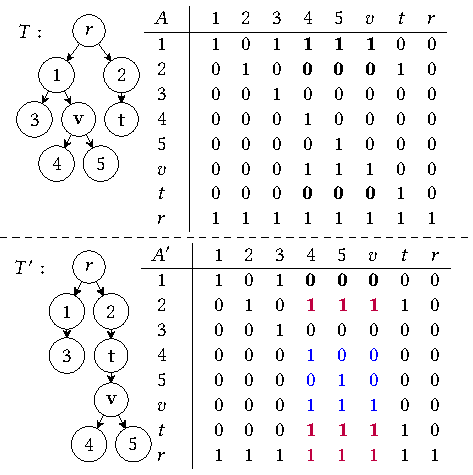
\includegraphics{figures/prune_reattach.pdf}
    \Description{A split figure with a mutation tree and its ancestor matrix on top and an altered version of the same mutation tree and its ancestor matrix below. In the altered tree, a node called ``v'' was detached from its previous parent and attached to another node called ``t;'' The ancestor matrix is changed accordingly.}
    \caption{Mutation tree and ancestor matrix representations before and after exemplary ``Prune and Reattach'' move where node $v$ is pruned from node $1$ and reattached to node $t$. Changes between $A$ and $A'$ marked in \textbf{bold}, \textcolor{emph}{colors} \textcolor{emph2}{highlight} partial rules to define $A'$.}
    \label{fig:prune_reattach}
\end{figure}

\begin{algorithm}
    \begin{algorithmic}[1]
        \STATE $A' \leftarrow 0 \in \{0,1\}^{|V| \times |V|}$
        \FORALL{$x \in V$}
            \STATE $Axt \leftarrow A[x][t]$ \COMMENT{Extract bit, 1 iff $x$ is ancestor of $t$}
            \STATE $Avx \leftarrow A[v][x]$ \COMMENT{Extract bit, 1 iff $v$ is ancestor of $x$}
            \FORALL[Parallel on complete bit-vector]{$y \in V$}  
                \IF{$A[v][y]$}\label{alg1:condition}
                    \STATE \COMMENT{Modify columns where $v$ is ancestor of $y$:}        
                    \STATE \COMMENT{\textcolor{emph2}{Connect via $t$} or \textcolor{emph}{retain subtree below $v$}}
                    \STATE $A'[x][y] \leftarrow \textcolor{emph2}{Axt} \vee \textcolor{emph}{(Avx \wedge A[x][y])}$\label{alg1:twocases}
                \ELSE
                    \STATE \COMMENT{Keep other columns}
                    \STATE $A'[x][y] \leftarrow A[x][y]$\label{alg1:keepaxy}
                \ENDIF
            \ENDFOR
        \ENDFOR
        \RETURN $A'$
    \end{algorithmic}
    \caption{Given a tree with nodes in $V$, represented as an ancestor matrix $A \in \{0,1\}^{|V| \times |V|}$, and nodes $v$ and $t$, compute the ancestor matrix $A'$ of the tree after the ``Prune and Reattach'' move with the parameters $v$ and $t$.}
    \label{alg:prune_reattach}
\end{algorithm}

In this section, we introduce the ``Prune and Reattach'' tree move as an example of the tree modification algorithms on ancestor matrices that we have developed for \ac{ffSCITE}. The other moves are similar in nature. For this move, two nodes $v$ and $t$ are sampled randomly. $v$ is sampled uniformly from all non-root nodes, but $t$ is sampled uniformly from all non-descendants of $v$ so that there is no path from $v$ to $t$ in the tree. Then, the node $v$ is moved from its current parent to node $t$. In other words, the entire subtree below $v$ is moved to a new parent. If there were a path from $v$ to $t$, the move would introduce a circle in the tree, which is why we sample $t$ from all non-descendants of $v$. Fig.~\ref{fig:prune_reattach} contains an example for this move, as well as the ancestor matrices of the tree before and after the move. In a parent vector encoding (not shown), only a single index would be changed, but in the ancestor matrix representation, multiple bits are different.

%Again, our goal now is to compute the ancestor matrix of the resulting tree from the original ancestor matrix and the move parameters. Alg.~\ref{alg:prune_reattach} builds the new ancestor matrix element by element. 
Given the inputs $A$ and the move parameters $v$ and $t$, the goal is to calculate $A'$ with simple bit-level operations. Alg.~\ref{alg:prune_reattach} presents our approach to build the new ancestor matrix element by element. 
For every pair of nodes $x$ and $y$, we find out whether there will be a path from $x$ to $y$ in the new tree. The answer to this question is the entry in the ancestor matrix for this pair. 
In the tree notation, the edge from the old parent of $v$ to $v$ is removed and a new edge from $t$ to $v$ is added. This means that the connectivity of $x$ and $y$ is only changed if the path between them would contain $v$. If there is no path from $v$ to $y$, then the potential path between $x$ and $y$ can not contain $v$. In this case, nothing changes and the entry from the old ancestor matrix is copied to the new one (Alg.~\ref{alg:prune_reattach}, lines~\ref{alg1:condition},~\ref{alg1:keepaxy}).
However, if there is a path from $v$ to $y$, then there are only two cases where a path from $x$ to $y$ can exist in the new tree: Either there is a path from $x$ to $t$, or the entire path between $x$ and $y$ is inside the subtree below $v$. If there is a path from $x$ to $t$, then we can construct a path from $x$ to $y$ via the newly introduced edge from $t$ to $v$, and if the path from $x$ to $y$ is entirely inside the subtree below $v$, then it is undisturbed by the move. The boolean expression $\textcolor{emph2}{Axt} \vee \textcolor{emph}{(Avx \wedge A[x][y])}$
%$Axt \vee (Avx \wedge A[x][y])$
(Alg.~\ref{alg:prune_reattach}, line~\ref{alg1:twocases}) covers exactly these cases, implicitly setting detached connections (in Fig.~\ref{fig:prune_reattach} the subtree below node $1$) and unrelated nodes (in Fig.~\ref{fig:prune_reattach} node $3$) to $0$.

Ancestor matrices are implemented as a list of bit vectors. The first index denotes a word in a RAM block and the second index denotes a bit in this vector. If we therefore fully unroll the inner loop over all nodes $y$, we get a single logic block that works on all bits of the vector in parallel. The hardware implementation first loads $A[v]$ to keep it in a register and then runs a single pipelined loop that loads $A[x]$, passes it through the logic, and stores the result in $A'[x]$. There are no loop-carried dependencies and the loop iteration space is fixed, unlike the ancestor matrix construction that this algorithm replaces. The other tree moves are implemented in the same way with a single pipelined loop with $|V|$ iterations and parallel logic operations per bit-vector word in the matrix.
%The other tree moves are implemented in the same way: Loading the old word from the ancestor matrix, applying combinatoric logic, and writing the results back. 
%Without these algorithms, an efficient implementation of \ac{SCITE} for \acp{FPGA} would not be possible.

\subsection{Likelihood computation}
\label{subsec:likelihood}

\begin{algorithm}[tbh]
    \begin{algorithmic}[1]
        \STATE $\mathrm{tree\_score} \leftarrow 0$
        \STATE $\mathrm{probability} \leftarrow [[\log(1-\alpha), \log(\beta)], [\log(\alpha), \log(1-\beta)]]$
        \STATE
        \FORALL[Pipelined sequentialy]{$c \in \mathrm{Cells}$}
            \STATE $\mathrm{max\_cell\_score} \leftarrow -\infty$
            \STATE
            \FORALL[Parallel, i.e. unrolled completely]{$v \in V$} \label{lst2:node_loop}
                \STATE $\mathrm{cell\_score} \leftarrow 0$
                \STATE
                \STATE \COMMENT{Cover all cases, unrolled completely}
                \FORALL{$\mathrm{prior}, \mathrm{posterior} \in \{0, 1\} \times \{0, 1\}$} \label{lst2:events_loop}
                    \STATE \COMMENT{Bit-vector load of known occurrences}
                    \STATE $\mathrm{v\_occurrences} \leftarrow \mathrm{is\_known}[c]$ 
                    \STATE
                    \STATE \COMMENT{Load and AND bit-vector of predicted cases}
                    \IF{$\mathrm{posterior} = 1$}
                        \STATE $\mathrm{v\_posterior} \leftarrow A^T[v]$
                    \ELSE
                        \STATE $\mathrm{v\_posterior} \leftarrow \neg A^T[v]$
                    \ENDIF
                    \STATE $\mathrm{v\_occurrences} \leftarrow \mathrm{v\_occurrences} \wedge \mathrm{v\_posterior}$
                    \STATE
                    \STATE \COMMENT{Load and AND bit-vector of reported cases}
                    \IF{$\mathrm{prior} = 1$}
                        \STATE $\mathrm{v\_prior} \leftarrow \mathrm{is\_mutated}[c]$
                    \ELSE
                        \STATE $\mathrm{v\_prior} \leftarrow \neg\mathrm{is\_mutated}[c]$
                    \ENDIF
                    \STATE $\mathrm{v\_occurrences} \leftarrow \mathrm{v\_occurrences} \wedge \mathrm{v\_prior}$
                    \STATE
                    \STATE \COMMENT{Compute and add score for this case}
                    \STATE $p \leftarrow \mathrm{probability}[\mathrm{posterior}][\mathrm{prior}]$
                    \STATE $\mathrm{case\_score} \leftarrow p \cdot \mathrm{popcount}(\mathrm{v\_occurrences})$ \label{lst2:popcount}
                    \STATE $\mathrm{cell\_score} \leftarrow \mathrm{cell\_score} + \mathrm{case\_score}$
                \ENDFOR
                \STATE
                \IF{$\mathrm{cell\_score} > \mathrm{max\_cell\_score}$}
                    \STATE $\mathrm{max\_cell\_score} \leftarrow \mathrm{cell\_score}$
                \ENDIF{}
            \ENDFOR
            \STATE $\mathrm{tree\_score} \leftarrow \mathrm{tree\_score} + \mathrm{max\_cell\_score}$
        \ENDFOR
        \RETURN $\mathrm{tree\_score}$
    \end{algorithmic}
    \caption{Given a tree with nodes in $V$, represented as an descendant matrix $A^T \in \{0,1\}^{|V| \times |V|}$, the mutation data matrices $\mathrm{is\_known}, \mathrm{is\_mutated} \in \{0, 1\}^{|\mathrm{Cells}| \times |V|}$, and the error probabilities $\alpha, \beta \in [0,1]$, compute the likelihood function from Subsection~\ref{subsec:likelihood}, as used in \ac{ffSCITE}.}
    \label{alg:likelihood_optimized}
\end{algorithm}

The same approach with parallel binary operations over bit-vectors and a pipelined loop over rows of the binary matrix is also applied to the likelihood calculation. 
%We have also exploited the properties of the bit-vector presentations to optimize the likelihood computation in Subsection~\ref{subsec:likelihood}: \todo{Rewrite to work without the naive implementation}
Since the original mutation matrix $D \in \{0, 1, 2\}^{|\mathrm{Cells}| \times |\mathrm{Genes}|}$ is not in a binary format, we instead encode it 
%In order to obtain simple binary operations in the central part of this computation, we encode the original mutation matrix $d \in \{0, 1, 2\}^{|\mathrm{Cells}| \times |\mathrm{Genes}|}$ 
with two binary matrices \texttt{is\_known} and \texttt{is\_mutated} $\in \{0, 1\}^{|\mathrm{Cells}| \times |V|}$. We define \texttt{is\_known}$[c][g] := (D[c][g] \neq 2)$ to encode whether the mutation status of a cell-gene combination is known, and define \texttt{is\_mutated}$[c][g] := (D[c][g] = 1)$ to encode the actual mutation status. These matrices are extended by one column such that the bit-vector format matches the one of the ancestor matrices. The \texttt{is\_known} entries for this extra column are $0$, such that it does not impact the likelihood value.
%First of all, we have transformed the input mutation matrix. Instead of using one mutation matrix $d \in \{0, 1, 2\}^{|\mathrm{Cells}| \times |\mathrm{Genes}|}$ with three possible values per cell, we use two matrices $\mathrm{is\_known}$ and $\mathrm{is\_mutated} \in \{0, 1\}^{|\mathrm{Cells}| \times |V|}$ with binary values. ``is\_known'' stores whether the mutation status of a cell-gene combination is known and ``is\_mutated'' stores the actual mutation status. We have also extended these matrices by one column so that we can use the same bit-vectors as for the ancestor matrices. This additional column, which represents the root node, is filled with unknown values so that it is not counted in the likelihood function.
%
Using these, calculating the likelihood of an attachment of a cell $c$ to a mutation tree node $v$ is possible with bit-wise logic operations. 
%With this modification, we can determine how often which event occurs by using bit-wise logic operations: Let's look at a cell $c$ which is attached to a node $v$. 
Looking at individual bits, we have a true positive mutation at gene $g$ if 
\begin{equation}
\texttt{is\_known}[c][g] \wedge \texttt{is\_mutated}[c][g] \wedge A^T[v][g]
\end{equation}
is true, which means that the cell-gene combination is reported as mutated and the underlying mutation tree model also reports the combination as mutated. 
%We have a true positive mutation at gene $g$ if $$\mathrm{is\_known}[c][g] \wedge \mathrm{is\_mutated}[c][g] \wedge A^T[v][g]$$ is true, which means that the cell-gene combination is reported as mutated and the underlying mutation tree model also reports the combination as mutated. 
Encoded as a complete bit-vector with word-level binary operations, the vector 
\begin{equation}
\label{eq:vector}
\texttt{is\_known}[c] \wedge \texttt{is\_mutated}[c] \wedge A^T[v]
\end{equation}
contains a $1$ bit for every true positive that has occurred for this cell and these occurrences can be counted with the so-called popcount function. Conversely, using the inverse $\neg\texttt{is\_mutated}[c]$ vector allows to find and count false positives, and using the inverse $\neg\mathrm{A^T[v]}$ for false respectively true negatives. The thus counted number of event occurrences is then multiplied by the respective logarithmic probability of the event and summed up to receive the log-likelihood of the entire cell attachment.
%This means that the bit-vector $$\mathrm{is\_known}[c] \wedge \mathrm{is\_mutated}[c] \wedge A^T[v]$$ contains a one for every true positive that has occurred for this cell. Conversely, the bit-vector $$\mathrm{is\_known}[c] \wedge \neg\mathrm{is\_mutated}[c] \wedge A^T[v]$$ contains a one for every false positive that has occurred for this cell, and so forth for the true and false negatives. If we count the ones in these bit-vectors with the so-called popcount function, we get the number of occurrences for every event, which we can multiply with the logarithmic probability of the event and sum up to receive the log-likelihood of the entire cell attachment.

Alg.~\ref{alg:likelihood_optimized} utilizes this way of computing the log-likelihood. The log-likelihood has the same ordering properties as the likelihood, but allows to replace exponentiation with multiplication (Alg.~\ref{alg:likelihood_optimized}, line~\ref{lst2:popcount}).
In order to find the most likely attachment of each cell to a node, the likelihood calculation of \ac{SCITE} as well as Alg.~\ref{alg:likelihood_optimized} originally contain three nested loops, one over cells, one over possible attachments (i.e. nodes in $A^T$) and one over genes per cell or node.
Following the vector-level notation of Eq.~\ref{eq:vector}, Alg.~\ref{alg:likelihood_optimized} replaces the loop over genes by bit-vectors that automatically yield parallel operations.
%In contrast to the reference outline in Alg.~??, the loop over all genes no longer shows up, because it is replaced by binary operations on bit-vectors and popcount invocations. 
On the other hand, to explicitly cover the four possible event classes with their respective \texttt{probability[posterior][prior]} values, Alg.~\ref{alg:likelihood_optimized} contains an explicit loop over all possible events (line~\ref{lst2:events_loop}). In order to generate parallel operations for these four classes, the loop is annotated with the unrolling attribute and will be specialized at compile time to the specific cases.
%Instead of summing up individual \texttt{probability[posterior][prior]} values, there is now only a single multiply-add step for each event class. On the other hand, Alg.~\ref{alg:likelihood_optimized} now contains a pair of explicit loops to iterate these four classes, which however after adding an unrolling attribute get fully evaluated at compile-time to form four separate datapaths, one for each class. 
To balance the throughput of the likelihood calculation with that of the other steps, we also mark the next loop dimension (line~\ref{lst2:node_loop}) with an unrolling attribute, which reduces the sequential steps of this function from cubic to linear, with a quadratically scaling bit-parallel datapath, which processes $4*|V|^2$ bits per clock cycle.
%replaced by bit-level AND and popcount operations and is therefore fully unrolled. The loops over the posterior and prior cases are unrolled too, which eliminates the case distinctions and the array accesses in the loop's body via constant propagation. This implementation of the log-likelihood function works exceptionally well on \acp{FPGA} due to its simplicity and we were also able to unroll one additional dimension. The resulting loop, which originally had a cubic runtime, therefore has a linear runtime and quadratic space utilization in \ac{ffSCITE}.


\section{Implementation and Evaluation}
\label{sec:evaluation}

\ac{ffSCITE} is implemented as a \ac{HLS} design written in C++20, using SYCL and Intel OneAPI version 22.3.0. %, which internally uses Intel Quartus version 20.4.0 Build 72 Pro. 
The target \ac{FPGA} is a Intel Stratix 10 GX 2800 \ac{FPGA} on a Nallatech 520N PCIe card. The utilized backend tool chain is Intel Quartus Pro version 20.4.0 Build 72, matching the version of the board support package (\emph{20.4.0\_hpc}) that provides PCIe and DDR memory interfaces. 
%The target \ac{FPGA} is a Intel Stratix 10 GX 2800 \ac{FPGA} on a Nallatech 520N, with the 20.4.0 HPC board support package.

\subsection{Hardware synthesis}
\label{subsec:hardware}


\begin{table*}[tbh]
    \centering
    \begin{tabular}{rllllllllll}
        \toprule
        \textbf{Kernel/Component} & \multicolumn{2}{l}{\textbf{Look-up tables}} & \multicolumn{2}{l}{\textbf{Flip-Flops}} & \multicolumn{2}{l}{\textbf{RAM blocks}} & \multicolumn{2}{l}{\textbf{MLABs}} & \multicolumn{2}{l}{\textbf{DSPs}} \\
        \cmidrule(r){1-1} \cmidrule(l){2-3} \cmidrule(l){4-5} \cmidrule(l){6-7} \cmidrule(l){8-9} \cmidrule(l){10-11}
        & \textbf{64-bit} & \textbf{96-bit} & \textbf{64-bit} & \textbf{96-bit} & \textbf{64-bit} & \textbf{96-bit} & \textbf{64-bit} & \textbf{96-bit} & \textbf{64-bit} & \textbf{96-bit} \\
        Static Partition & 24.4\% & 24.4\% & 24.4\% & 24.4\% & 22.4\% & 22.4\% & 0.0\% & 0.0\% & 18.2\% & 18.2\% \\
        Interconnect & 1.2\% & 1.2\% & 0.7\% & 0.7\% & 1.0\% & 0.9\% & 0.0\% & 0.0\% & 0.0\% & 0.0\% \\
        IO Kernel & 0.7\% & 0.6\% & 0.6\% & 0.6\% & 0.8\% & 0.6\% & <0.1\% & <0.1\% & <0.1\% & <0.1\% \\
        Worker Kernel & 16.4\% & 27.7\% & 10.5\% & 13.6\% & 6.5\% & 10.8\% & 1.0\% & 0.6\% & 9.8\% & 12.6\% \\
        % Blocks B8, B9
        \textit{(thereof ``Execute Move'')} & \textit{(9.2\%)} & \textit{(13.6\%)} & \textit{(5.4\%)} & \textit{(6.3\%)} & \textit{(3.0\%)} & \textit{(2.9\%)} & \textit{(0.6\%)} & \textit{(0.3\%)} & \textit{(8.0\%)} & \textit{(10.8\%)} \\
        \textbf{Total} & \textbf{42.7\%} & \textbf{53.9\%} & \textbf{36.2\%} & \textbf{39.4\%} & \textbf{30.7\%} & \textbf{34.9\%} & \textbf{1.0\%} & \textbf{0.6\%} & \textbf{28.0\%} & \textbf{30.8\%} \\
        \bottomrule
    \end{tabular}
    \Description{A table with the resource usages of the different parts of the two designs. The listed resources are look-up tables, flip-flops, RAM blocks, MLABs, and DSPs, and the listed parts are the static partition, the interconnect, the IO kernel, the worker kernel, and thereof the ``Execute Move'' block.}
    \caption{Resource usage of the 64-bit and 96-bit design instances. The 64-bit instance is clocked at 307.50 MHz, and the 96-bit instance is clocked at 316.67 MHz. Percentages are relative to available resources on the Intel Stratix 10 GX 2800 \ac{FPGA} (1866240 look-up tables, 3732480 flip-flops, 11721 RAMs, $\sim$133900 MLABs, 5760 DSPs). The static partition provides the interface to the host and is fixed by the card vendor.}
    \label{tab:ressource_usage96}
\end{table*}

All components inside the worker kernel (Sec.~\ref{sec:kernel_structure}) are implemented as pipelined loops with an \ac{II} of 1 that iterate over the tree nodes. The maximal number of nodes in a tree is fixed as a design parameter during compilation. This means that the number of bits in a bit-vector, the number of vectors in an ancestor matrix, and therefore also the number of iterations and the width of the data path are fixed with this parameter. The biggest vector size that we have found to be reliably synthesizable for this target is 96 bits; The resource usage for such a design instance as well as for a smaller 64-bit variant is listed in Tab.~\ref{tab:ressource_usage96}. Both designs are relatively logic-intensive, on the one hand due to many bit-level operations, mostly in the ``Execute Move'' loop, and on the other hand to orchestrate movement of the bit-matrices. The floating-point \acp{DSP} of the Stratix 10 architecture see some usage for the arithmetic parts of the likelihood calculation, and not many \acl{BRAM} are used. Despite different resource usage, both designs achieve similar clock frequencies around 310 MHz.

The bottleneck for larger vector sizes is routing. When trying to compile the design with 128-bit vectors with an unlimited clock speed, the demand for interconnect wires peaks up to 125\%. This is only eliminated by lowering the clock speed to the regions around 150 MHz, which is less than a third the maximum clock speed of 480 MHz for the Intel Stratix 10 \ac{FPGA} and less than half the clock speeds of the smaller design instances. Even with a lowered clock speed, timing errors still occur and we were thus unable to reliably synthesize the design with 128 bits. There also seems to be an issue with the arbitrary precision integer type\footnote{\url{https://www.intel.com/content/www/us/en/docs/oneapi-fpga-add-on/optimization-guide/2023-0/var-prec-fp-sup.html}} that we use to implement bit vectors. The last bit of the 96-bit vector is always set to zero and thus limits the usable number of nodes in our experiments to 95. The problem does not show up with 32-bit, 64-bit, or spurious 128-bit design instances.


\subsection{Performance benchmark}
\label{subsec:performance}

In order to compare the performance of \ac{ffSCITE} to the reference \ac{SCITE} implementation by \citeauthor{tree2016} \cite{tree2016}, we measure the throughput in Markov chain steps per second.
%Our main goal is to provide an implementation of \ac{SCITE} that has a higher throughput in Markov chain steps per second than the reference implementation by \citeauthor{tree2016} \cite{tree2016}. We have set up the following benchmark to verify that we have met this goal: 
For this benchmark, we have generated random input data with different sizes, using the stochastic assumptions presented in Section \ref{sec:introduction} and arbitrary error probabilities. We wanted to test both \ac{ffSCITE} variants with fully and partially utilized bit vectors and therefore chose 32 bits, 64 bits, and 95 bits as input sizes. For 32 bits, the input covers 32 cells and 31 genes so that the mutation tree has 32 nodes. Other input sizes are analogous, and we had to use 95 bits as the biggest input size since the 96th bit of 96-bit \ac{ffSCITE} is faulty (see Subsection \ref{subsec:hardware}). Then, we simulated 48 Markov chains with 2,000,000 chain steps each for every input and measured the runtime, as well as the power draw of the \ac{ffSCITE} instances. We repeated this experiment four times and took the average of those repetitions as the final value.

\begin{table}[tbh]
    \begin{tabular}{crrrcc}
        \toprule
        \textbf{Input Size}
        & \multicolumn{3}{c}{\textbf{Throughput [ksteps/s]}} 
        & \multicolumn{2}{c}{\textbf{Speedup}} \\
        \cmidrule(r){1-1}
        \cmidrule(r){2-4}
        \cmidrule(r){5-6}
        \textbf{Cells $\times$ Genes}
        & \textbf{CPU} 
        & \multicolumn{2}{c}{\textbf{FPGA design}}
        & \multicolumn{2}{c}{\textbf{FPGA/CPU}} \\
        \cmidrule(r){3-4}
        \cmidrule(r){5-6}
        & & \textbf{96-bit} & \textbf{64-bit} & \textbf{96-bit} & \textbf{64-bit} \\
        32 $\times$ 31 & 229.87 & 4891.25 & 7486.57  & 21$\times$ & 33$\times$ \\
        64 $\times$ 63 &  70.65 & 4123.53 & 4349.70  & 58$\times$ & 62$\times$ \\
        95 $\times$ 94 &  36.55 & 2938.25 & n/a      & 80$\times$ & n/a \\
        \bottomrule
    \end{tabular}
    \Description{A table listing the throughput of the CPU reference as well as the 96-bit and 64-bit designs in ksteps/s for different input sizes. The input sizes are 32 cells and 31 genes, 64 cells and 63 genes, and 95 cells and 94 genes. Additionally, the speedup of the FPGA designs relative to the CPU reference is listed.}
    \caption{Mean throughput of SCITE (single thread on AMD EPYC Milan 7763 CPU) and two variants of \ac{ffSCITE} (Stratix 10 GX 2800 FPGA) for different input sizes. 64-bit \ac{ffSCITE} is not able to process mutation matrices with more than 63 genes since the bit vector width limits the number of genes it can process. 
    %96-bit \ac{ffSCITE} constantly draws 75.17 W and 64-bit \ac{ffSCITE} constantly draws 72.42 W.
    }
    \label{tab:throughput}
\end{table}

This performance data is shown in Tab.~\ref{tab:throughput}, where we have listed the throughput of the three executables in executed Markov chain steps per second. We see that both \ac{ffSCITE} variants are significantly faster than the CPU-based \ac{SCITE} implementation, with speedups of up to 80$\times$. We also see that the speedup grows %nearly linearly 
with the input size and that the smaller \ac{ffSCITE} variant achieves a higher throughput for the inputs it can process than the bigger variant, despite slightly lower clock frequency. This means that if a user knows that their input will not exceed a certain synthesizable size, it can be beneficial to only build \ac{ffSCITE} with this bit-vector length.

\subsection{Performance model and pipeline latency}

\begin{table}[tbh]
    \begin{tabular}{cccccc}
        \toprule
        \textbf{Instance} & \textbf{Input Size} & \multicolumn{2}{c}{\textbf{Throughput [ksteps/s]}} & \textbf{Acc.} \\
        \cmidrule(r){1-1} \cmidrule(r){2-2} \cmidrule(r){3-4} \cmidrule(r){5-5}
        & \textbf{Cells $\times$ Genes} & \textbf{Measured} & \textbf{Modelled} \\
        96-bit & 32 $\times$ 31 & 4891.25 & 9596.06 & 51.0\% \\
        & 64 $\times$ 63 & 4123.53 & 4871.85 & 84.6\% \\
        & 95 $\times$ 94  & 2938.25 & 3298.65 & 89.1\% \\
        64-bit & 32 $\times$ 31 & 7486.57 & 9318.18 & 80.3\% \\
        & 64 $\times$ 63 & 4349.70 & 4730.77 & 91.9\% \\
        \bottomrule
    \end{tabular}
    \Description{A table listing the measured throughput and the model prediction for the different design instances and input sizes.}
    \caption{Comparison of measured and modeled throughput for different design instances and input sizes, including the model accuracy.}
    \label{tab:model}
\end{table}

The throughput of \ac{ffSCITE} can be modeled by the number of iterations in its pipelined loops, ideally consuming one cycle per iteration. The slowest of these loops transfers the current state of a chain between IO and worker kernel.
%The throughput of \ac{ffSCITE} is bounded by its design with separate IO and worker kernels: 
%The current state of a chain is transferred between these kernels via pipes, but this state is too big to be transferred in one clock cycle. 
Each state is therefore transferred in packets, row by row. With $n$ denoting the number of nodes in the mutation tree (i.e. the number of utilized bit-vector bits and rows in an ancestor matrix), then the first $n$ packets contain a tuple with a row of the ancestor matrix and a row of the descendant matrix, followed by one packet with meta information. In total, there are $n+1$ packets per state, which takes $n+1$ cycles to be transferred. The other pipelined loops, i.e. the likelihood calculation and the mutation tree updates, should be slightly faster at $n$ cycles.
Thus, the throughput of the pipe in steps per second is upper bounded by $f/(n+1)$ in steps per second, where $f$ is the clock frequency of the final design.

We compare the measured throughput of \ac{ffSCITE} with this model in Tab.~\ref{tab:model}. The model matches fairly well for inputs that fully utilize the available bit-vectors, but the model accuracy drops off for smaller inputs. We suspect that this might be due to the overall latency of the worker kernel: The IO kernel currently assumes a fixed latency of the worker kernel, measured in chain states, which does not take the input size into account. However, the worker's latency in processed chain states might be bigger for smaller input sizes. This would mean that the IO kernel needs to stall until the results are sent back from the worker, which would explain the lowered throughput. This hypothesis could be investigated with further experiments. %Unfortunately, we have not properly tested this hypothesis yet. 
The presented designs are based on a coarse empirical design space exploration, which yielded 24 independent chain states to hide the worker latency.
%We have only made a coarse design space exploration to find the worker latency with the highest throughput, which yielded 24 chain states as the best approximation. 
The good correspondence of measurements and model for full inputs confirms that this choice is reasonable for this case, but may need refinement for other input sizes.
%However, the good accuracy of the model for full inputs is enough for us to use this model as an idealized upper bound of \ac{ffSCITE}'s performance.
\section{Analysis with Idealized CPU Reference}
\label{subsec:cpu}

In Subsection \ref{subsec:performance}, we have shown that \ac{ffSCITE} achieves up to 80$\times$ the throughput of the CPU reference implementation by \citeauthor{tree2016} \cite{tree2016}. 
This is a good result, but strongly influenced by limited performance engineering done for the reference.
%This is an achievement, but we have to be fair and admit that the reference implementation is not very well optimized. 
In particular, it does not make use of multi-threading to parallelize the work and also uses many memory allocation calls within loop kernels. In this section, we try to assess how \ac{ffSCITE} could compare to a highly optimized CPU version, without undergoing the CPU optimization effort for the full application. Therefore, we focus on the likelihood calculation as a synthetic proxy to upper-bound the optimized CPU throughput.
%We wanted to know how \ac{ffSCITE} would compare to an optimized version of \ac{SCITE} for CPUs, but no one has published such an implementation to the best of our knowledge. Optimizing \ac{SCITE} for CPUs was outside the scope of our work too, so we decided to create a synthetic benchmark to estimate the throughput an optimized version of \ac{SCITE} could achieve on CPUs.

Our synthetic benchmark runs the log-likelihood computation (Alg.~\ref{alg:likelihood_optimized}) on mutation matrices with 128 cells and 127 genes: It first loads the mutation data matrix and prepares the initial Markov chain states like a functional implementation of \ac{SCITE}. However, it only repeatedly computes the likelihood score of these initial states and never modifies them. 
We chose the log-likelihood function as our kernel since it is the part of the algorithm with the fastest-growing runtime and also consumes a significant resource fraction of the FPGA designs.
%We chose the log-likelihood function as our kernel since it is the part of the algorithm with the fastest-growing runtime and since all operations inside the loop body are available as x86 instructions, even the popcount function. We therefore assume that the benchmark provides a good upper bound for the best possible performance of \ac{SCITE} on CPUs. 
In contrast to the largest evaluated FPGA design with 96 bits, we chose 128 cells and 127 genes as the input size, since power-of-two dimensions often enable more efficient CPU execution, in particular when vector operations are used.
%since 64 cells and 63 genes are less than what 96-bit \ac{ffSCITE} supports and 95 cells and 94 genes would be harder to implement efficiently. 
The benchmark is also implemented in C++ using SYCL and Intel OneAPI and shares much of the non-performance-critical code with \ac{ffSCITE}.

\begin{table*}[tbh]
    \begin{tabular}{lcrrr}
        \toprule
        \textbf{Hardware (Design)} & \multicolumn{1}{c}{\textbf{Input Size}} & \textbf{Throughput} & \textbf{Power Draw} & \textbf{Energy Consumption}\\
        & \textbf{[cells $\times$ genes]} & \textbf{[counted Tbit/s]} & \textbf{[W]} & \textbf{[pJ/counted bit]}\\
        \cmidrule(r){1-1} \cmidrule(lr){2-2} \cmidrule(r){3-3} \cmidrule(r){4-4} \cmidrule(r){5-5}
        2x AMD EPYC Milan 7763 & 128 $\times$ 127 & 18.88 & 556.05 & 29.45 \\
        1x Stratix 10 GX 2800 (96-bit) & 95 $\times$ 94 & 10.08 & 75.17 & 7.46 \\
        1x Stratix 10 GX 2800 (64-bit) & 64 $\times$ 63 & 4.56 & 72.42 & 15.88 \\
        2x Intel Xeon Gold 6148 & 128 $\times$ 127 & 1.95 & \textit{*300.00} & \textit{*153.85} \\
        \bottomrule
    \end{tabular}
    \Description{A table listing the throughput in counted bits per second of the AMD EPCY Milan 7763 CPU, the 96-bit and 64-bit \ac{ffSCITE} designs, and the Intel Xeon Gold 6148 CPU, as well as their power draw and energy consumption per counted bit.}
    \caption{Comparison of synthetic log-likelihood calculation on CPU vs. full \ac{ffSCITE} on FPGA.
    %evaluated popcount bits per second on different hardware. Note that only the throughput of a single CPU chip is listed, not the throughput of an entire node. 
    Power and energy numbers based on measured power consumption, except for \textit{*marked} numbers based on nominal  TDP.}
    \label{tab:counted_bits}
\end{table*}

We ran the benchmark on individual nodes of the two supercomputers Noctua~1 and Noctua~2, hosted at the Paderborn Center for Parallel Computing.
Noctua~1 nodes, installed in 2018, contain 2 Intel Xeon Gold 6148 CPUs that are manufactured with the same 14 nm technology as the Intel Stratix 10 GX 2800 \ac{FPGA} we used for \ac{ffSCITE}. 
Noctua~2 nodes contain 2 AMD EPYC Milan 7763 CPUs, representing a high-end server CPU platform in 2022.
%Noctua~1 nodes have the older and smaller Intel Xeon Gold 6148 CPUs compared to Noctua~2's AMD EPYC Milan 7763 CPUs, but they are manufactured with the same 14 nm technology as the Intel Stratix 10 GX 2800 \ac{FPGA} we used for \ac{ffSCITE}. 
Most of the operations in the loop body can be vectorized except for the popcount instruction. This means that in a vectorized implementation of the log-likelihood function, the vectors are completely unpacked for the popcount operations and are then repacked afterwards. With the 512-bit vector registers of the Noctua~1 nodes, the total number of executed instructions is reduced in comparison to a scalar implementation, but with the 256-bit vector registers of the Noctua~2 nodes, this is not the case. We have therefore decided to use the respectively faster vectorized implementation for Noctua~1 and the scalar implementation for Noctua~2. Apart from this, we have used the IntelLLVM compiler version 2022.2 for Noctua~2 and version 2022.2.1 for Noctua~1. The compiler arguments were
\begin{center}
    \texttt{-O3 -DNDEBUG -qactypes -std=gnu++20 -fsycl-targets=spir64\_x86\_64-unknown-unknown}
\end{center}
for all operations, and additionally
\begin{center}
    \texttt{-Xsdevice=\allowbreak cpu} \texttt{-Xsmarch=\allowbreak avx2}
\end{center}
for linking on Noctua~2, and 
\begin{center}
    \texttt{-Xsdevice=\allowbreak cpu} \texttt{-Xsmarch=\allowbreak avx512}
\end{center}
for linking on Noctua~1.

For the $128 \times 127$ inputs, one entire Noctua~2 node achieves a throughput of 2251.02 ksteps/s and one entire Noctua~1 node achieves 233.05 ksteps/s. Both systems are utilized very well: Noctua~1 achieves an L1D miss-rate of 0.03\% and an IPC of roughly 1.87, while Noctua~2 even achieves an L1D miss-rate of 0.005\% and an IPC of roughly 5.1. We assume that there may be some more optimization possible by reducing the number of instructions, but we should also stress that this performance does not even cover the entire Markov chain step % and that every node contains two separate CPUs. 

Since the throughput in ksteps/s varies on all architectures with different input sizes, as seen in Section~\ref{subsec:performance}, we also need to normalize between the synthetic CPU benchmark and the full \ac{ffSCITE} measurements. 
%The question remains how this benchmark compares to \ac{ffSCITE}. To normalize the throughput figures for the different input sizes, 
To this end, we introduce the metric of counted bits per second. %: An integral part of the likelihood computation is the popcount instruction. Other operations could be optimized away or implemented differently, but the popcount operation is always necessary. 
Every chain step requires preparing and counting the $1$s in $4 \times n^3$ bits where $n$ is the number of cells and the number of bits in a bit-vector. By multiplying the number of counted bits per chain step with the measured throughput in steps per second, we obtain the performance figures in Tab.~\ref{tab:counted_bits}. When comparing individual chips, we see that 96-bit \ac{ffSCITE} performance is en-par with a single AMD EPYC Milan CPU (note that Tab.~\ref{tab:counted_bits} presents numbers for the entire node) and outperforms a single Intel Xeon Gold CPU by an order of magnitude. 
Looking at power measurements and energy efficiency, we see that the two EPYC Milan CPU per node consume around 7.5$\times$ more power than a single FPGA board. Normalized to energy consumption per counted bit, with 7.5 pJ/bit the FPGA architecture is around 4$\times$ more energy efficient than the EPYC Milan CPU at 29.5 pJ/bit.
%We have also measured the power draw of the Noctua~2 node during execution, and its energy consumption per counted bit is almost four times the energy consumption of 96-bit \ac{ffSCITE}. There are no power measurements available for Noctua 1, but since the measurements for Noctua 2 are constantly slightly over its TDP, we assume this for Noctua 1 too.


\section{Related Work}

Typical FPGA accelerators for bioinformatics workloads~\cite{yu-kw-03a,zh-ta-07a,ja-la-08a} rely solely on highly data-parallel datapaths with customized bit-width. Similar to our work, Guo et al.~\cite{gu-la-19a} additionally consider an iterative step for a form of chain expansion around the data-parallel core. With this, they also encounter a latency challenge on the feedback of this step. Orthogonal to our solution of overlapping this latency with steps from other chains, they focus on minimizing the latency of the individual step by reordering the computation order.

On the algorithmic side, Kuipers et al.~\cite{ku-ja-17a} have extended the search space for possible mutation trees by softening the infinite-site assumption. This allows to reconstruct some mutation histories more accurately and could be considered in possible extensions of \ac{ffSCITE}.

\section{Conclusion and Future Work}

In this work, we have introduced \ac{ffSCITE}, an \ac{FPGA} design and implementation of the \ac{SCITE} algorithm that outperforms the original CPU reference by up to 80$\times$. % that is optimized for high-level \ac{FPGA} designs. 
%We have introduced \ac{ffSCITE}, an implementation of the \ac{SCITE} algorithm that is optimized for high-level \ac{FPGA} designs. 
For inputs matching the design parameters, a performance model illustrates the good occupancy of the FPGA design.
%The resulting design is utilized well and performs the same workloads up to 80 times as fast as the original reference implementation for CPUs. 
We have also approximated the maximum performance that an optimized CPU implementation can achieve for one of the core loops of \ac{ffSCITE}. Even here, the FPGA performance is en-par with current high-performance CPUs at much lower power consumption, while outperforming CPUs of the same manufacturing technology by an order of magnitude.

We see several directions for future work. A main limitation of the current design are the maximal input and mutation matrix sizes fixed at compile-time. A blocking approach could open up the design for arbitrarily large inputs, possibly at the cost of decreased performance.
On the other hand, since the presented designs still leave a signification fraction of FPGA resources unused, there could be headroom for further performance improvements, for example via replications of the worker kernel.

%We can see multiple directions for future work: First of all, we are certain that even more throughput could be achieved by replicating the entire design. Even the 96-bit \ac{ffSCITE} instance only utilizes 29\% of all \acp{LUT} and has 46\% to spare for one or maybe two replications to double or triple the end-to-end throughput. Additional resource-saving optimizations on lower levels could increase this speedup even further. Another fundamental limitation of the design is the fixed input and mutation matrix sizes. Further developments could open up the design for arbitrarily large inputs, possibly at the cost of decreased performance.


\bibliographystyle{ACM-Reference-Format.bst}
\bibliography{literature} 

\end{document}
\endinput
%%
%% End of file `sample-authordraft.tex'.
